\documentclass[11pt,a4paper]{article}

% ------------------------------------------------------------------
% Packages
% ------------------------------------------------------------------
\usepackage[T1]{fontenc}
\usepackage[utf8]{inputenc}
\usepackage{lmodern}
\usepackage[a4paper,margin=2.0cm,headheight=14pt]{geometry}
\usepackage{microtype}
\usepackage{amsmath,amssymb}
\usepackage{booktabs}
\usepackage{tabularx}
\usepackage{array}
\usepackage{enumitem}
\usepackage{xcolor}
\usepackage{fancyhdr}
\usepackage{titlesec}
\usepackage{caption}
\usepackage{float}
\usepackage[most]{tcolorbox}
\usepackage{tikz}
\usetikzlibrary{arrows.meta,positioning,fit,backgrounds,calc}
\usepackage[colorlinks=true,linkcolor=navy,urlcolor=navy]{hyperref}

% ------------------------------------------------------------------
% Colours
% ------------------------------------------------------------------
\definecolor{secblue}{HTML}{2B5B8A}
\definecolor{navy}{HTML}{1A1A80}
\definecolor{lightblue}{HTML}{EAF1F8}
\definecolor{boxblue}{HTML}{2E5C8A}
\definecolor{gaporange}{HTML}{C0661A}
\definecolor{gapfill}{HTML}{FCEFE3}
\definecolor{goodgreen}{HTML}{2E8B57}
\definecolor{goodfill}{HTML}{E9F7EE}
\definecolor{badred}{HTML}{C0392B}
\definecolor{badfill}{HTML}{FDECEC}

% ------------------------------------------------------------------
% Layout
% ------------------------------------------------------------------
\titleformat{\section}{\color{secblue}\large\bfseries}{\thesection}{0.6em}{}
\titleformat{\subsection}{\color{secblue}\normalsize\bfseries}{\thesubsection}{0.6em}{}
\titlespacing*{\section}{0pt}{10pt}{4pt}
\titlespacing*{\subsection}{0pt}{7pt}{3pt}

\pagestyle{fancy}
\fancyhf{}
\fancyhead[L]{\small LMA Group Project 2026 --- Proposal Brief}
\fancyhead[R]{\small Negotiate, Then Solve}
\fancyfoot[C]{\small\thepage}
\renewcommand{\headrulewidth}{0.4pt}

\captionsetup{font=small,skip=3pt}
\setlist[itemize]{itemsep=2pt,topsep=3pt,leftmargin=1.4em}
\setlist[enumerate]{itemsep=1pt,topsep=2pt}
\setlength{\parskip}{3pt}
\setlength{\textfloatsep}{8pt}
\setlength{\floatsep}{6pt}
\setlength{\intextsep}{6pt}
\makeatletter
\setlength{\@fptop}{0pt}
\makeatother
\usepackage{needspace}
\newcolumntype{L}[1]{>{\raggedright\arraybackslash}p{#1}}
\newcolumntype{Y}{>{\raggedright\arraybackslash}X}

\newtcolorbox{keybox}{enhanced,colback=gapfill,colframe=gaporange,
  boxrule=1pt,arc=3pt,left=6pt,right=6pt,top=3pt,bottom=3pt}
\newtcolorbox{bluebox}[1]{enhanced,colback=lightblue,colframe=boxblue,
  coltitle=white,fonttitle=\small\bfseries,title={#1},boxrule=0.8pt,arc=3pt,
  left=6pt,right=6pt,top=3pt,bottom=3pt}

\tikzset{
  >=Stealth,
  arr/.style={->,draw=boxblue,thick},
  fb/.style={->,draw=gaporange,dashed,thick},
}

\newcommand{\stepno}[1]{{\color{secblue}\textbf{#1.}}}
\newcommand{\circled}[1]{\tikz[baseline=(c.base)]\node[circle,fill=secblue,text=white,font=\tiny\bfseries,inner sep=0pt,minimum size=10pt](c){#1};}

% ==================================================================
\begin{document}

% ------------------------------------------------------------------
% Title block
% ------------------------------------------------------------------
\begin{center}
{\color{secblue}\rule{\textwidth}{0.8pt}}\par\vspace{2pt}
{\Large\bfseries Negotiate, Then Solve\par}
\vspace{2pt}
{\large Solver-Grounded Negotiation for Conflict-Aware University Timetabling\par}
\vspace{2pt}
{\color{secblue}\rule{\textwidth}{0.8pt}}\par
\vspace{3pt}
{\small\textbf{Domain:} institute management (academic timetabling)\\
\textbf{Target users:} academic office, Dean / HoD, faculty, lab in-charges and exam cell, students\\
\textbf{Capabilities:} fine-tuning, RAG, reasoning, agentic abilities, tool calling\\
\textbf{Team Farali Chevdo}\\[2pt]
\begin{tabular}{@{}l@{\;\;}l@{\qquad}l@{\;\;}l@{}}
Achyutananda Sahoo & 2025202028 & Rakesh C & 2026901015\\
Satyajit Priyadarshi & 2025201055 & Shubhadeep Mandal & 2025201056\\
\end{tabular}\par}
\end{center}

\noindent\textbf{Abstract.} {\small University timetables change constantly
after publication, and change requests arrive as unstructured text. LLMs can
read such requests but do not provide a formal guarantee of hard-constraint
satisfaction; constraint
solvers guarantee validity but cannot read requests, explain infeasibility or
negotiate. We study \emph{solver-grounded negotiation}: when requests are
infeasible, minimal unsatisfiable subsets (MUS) locate the conflict, minimal
correction sets (MCS) define the candidate concessions, and OR-Tools CP-SAT
re-solves each relaxation into a concrete timetable. An LLM negotiator may
offer \emph{only} these solver-verified options, ranked by a published
priority policy and a concession ledger, and explains each in terms traceable
to solver evidence. A human coordinator approves every change. We compare
against the same agent negotiating with LLM-invented alternatives, both
unverified and filtered by the same solver, on planted-conflict scenarios
with stakeholder simulators that hide their true flexibility.\par}

% ------------------------------------------------------------------
\section{Problem and Motivation}
% ------------------------------------------------------------------
A university timetable is built once per semester but changes weekly.
Faculty report unavailability, labs close for maintenance, guest lecturers
arrive with fixed windows and students report elective clashes. These
requests arrive as unstructured text through the portal, email and messaging
apps, and the academic office resolves them by hand; one change often
silently breaks another constraint. When two requests cannot both be
satisfied, there is no systematic way to decide \emph{who should concede},
so decisions look arbitrary to those affected. Existing tools either
check a finished timetable or rebuild it from scratch; none reads the
request, explains why it cannot be met, or negotiates who gives way.

\noindent\textbf{Why it matters.} A single double-booked room disrupts whole
sections for weeks, most requests have a safe resolution that could be
found in seconds, and stakeholders accept compromises more readily when they
can see why one was chosen and that concessions rotate.

\subsection{Domain and Target Users}
\textbf{Domain:} institute management systems, specifically academic course
timetabling, scoped to one department ($\approx$30 faculty, 60 sections, 20
rooms, 5-day $\times$ 8-slot week). \textbf{Target users} are five
stakeholder groups with different needs and authority; their authority
determines who may relax which tier of constraint (Section~\ref{sec:mech}).
\begin{table}[H]
\centering\small
\begin{tabularx}{\textwidth}{@{}l Y l@{}}
\toprule
\textbf{Stakeholder} & \textbf{What they need from the system} & \textbf{Authority}\\
\midrule
Coordinator (academic office) & Verified changes and conflict summaries & Approves and publishes\\
Dean / HoD & Short briefs for policy exceptions and deadlocks & Dean: T1 policy; HoD: dept.\\
Faculty (incl.\ visiting) & Plain-language requests; explained outcomes & Own classes only\\
Lab in-charge, exam cell & Report outages; protect exam blocks & Rooms; T2 calendar blocks\\
Students / class reps & Report clashes and get a tracked response & Raise issues only\\
\bottomrule
\end{tabularx}
\end{table}

\subsection{What Is Missing}
\begin{table}[!htb]
\centering\small
\begin{tabularx}{\textwidth}{@{}L{4.6cm} Y@{}}
\toprule
\textbf{Approach} & \textbf{Limitation for this problem}\\
\midrule
Classical timetabling solvers (CP/MIP) & Need fully formal constraints; cannot read requests, explain infeasibility or negotiate\\
LLM scheduling directly & Reads plain language but may violate hard constraints; no formal feasibility guarantee\\
LLM + solver (verifier) & Solver checks LLM output; a filter drops infeasible ideas, but candidates are still whatever the LLM imagines, so valid concessions can be missed\\
LLM negotiation agents & Free-form offers with no model of what is feasible\\
MUS/MCS infeasibility diagnosis & Finds minimal conflicts and repairs, but serves a single modeller; no multi-stakeholder negotiation\\
\bottomrule
\end{tabularx}
\end{table}
Prior approaches provide several of these components individually. What is
missing in our setting is an \emph{interpretation layer} that connects formal infeasibility analysis to
multi-stakeholder negotiation: deciding which concessions are possible, whom
to ask, and how to explain it, without ever leaving the feasible space.

% ------------------------------------------------------------------
\section{Research Question and Hypotheses}
\label{sec:rq}
% ------------------------------------------------------------------
\begin{keybox}
\textbf{RQ.} Can solver-derived conflict sets constrain an LLM negotiator so
that it resolves infeasible timetable requests with \emph{fewer negotiation
rounds} and \emph{lower disruption} than LLM-invented options, even when
those options are filtered by the same solver before they are offered?
\end{keybox}
\noindent By construction, our system never offers an infeasible option;
this is a design property, not a hypothesis. The open question is whether
that guarantee is worth its price: restricting options to MCS relaxations
may miss creative alternatives (a third-party swap, an unusual slot) that a
free-form LLM could find and a stakeholder would accept.
\begin{itemize}
  \item \textbf{H1 (cost of invented candidates).} Unverified LLM options (B3)
  are solver-rejected often enough to cost extra rounds and escalations;
  filtered LLM options (B4) avoid that but need more regeneration calls and
  miss concessions that MCS enumeration covers.
  \item \textbf{H2 (efficiency and quality).} Against B4, ours achieves an
  equal or higher resolution rate with fewer rounds, less disruption and a
  smaller gap to an unrestricted oracle that knows every stakeholder's hidden
  flexibility.
  \item \textbf{H3 (explanation).} Explanations grounded in the conflict set
  are more faithful than free-form explanations of the same options: more
  claims trace to a fact, fewer private reasons leak, and the text never
  describes an option that was not offered, without lowering acceptance.
  The human pilot rates clarity and acceptability.
  \item \textbf{H4 (fairness).} The concession ledger lowers the dispersion
  of concession burden across stakeholders (Gini, maximum individual burden)
  compared with flat weights, without lowering the resolution rate.
\end{itemize}
A scenario is \emph{resolved} when every affected stakeholder accepts an
offered alternative and the combined repair re-solves feasibly; otherwise it
is \emph{escalated} (deadlock, timeout, or a Tier~1--2 option). Every system
reports resolution rate, rounds-given-resolution and escalation rate
together, so no system can look efficient by escalating hard cases early.
Hypotheses are directional; we report effect sizes with 95\% bootstrap
confidence intervals and paired tests, and negative results will be
reported.

% ------------------------------------------------------------------
\section{Proposed Approach}
% ------------------------------------------------------------------
Figure~\ref{fig:arch} follows one request through the system:
\textbf{Request $\to$ Parse $\to$ Policy check $\to$ Solve $\to$ Negotiate
$\to$ Human approval}. Steps \circled{1}--\circled{4} turn a plain-language
message into a checked constraint model; step \circled{5} is the research
contribution; step \circled{6} keeps a human in control of publication.

\begin{enumerate}[label=\protect\circled{\arabic*},leftmargin=2em]
  \item \textbf{Receive.} Each channel produces one \texttt{Request} record
  with the sender's identity and role (experiments inject synthetic requests
  here).
  \item \textbf{Parse.} A router sends routine requests to a small
  LoRA-tuned compiler and ambiguous ones to the prompted base model; both emit the same
  typed constraint JSON. A deterministic authority check, not a model,
  decides whether the sender may make the request.
  \item \textbf{Policy check.} Retrieved institute rules classify the request
  as allowed, needs approval or forbidden, with a citation.
  \item \textbf{Solve.} CP-SAT models room, faculty, student-group and
  institutional constraints and repairs the published timetable with as few
  changes as possible. Each request constraint is guarded by an assumption
  literal so it can be switched off. Feasible repairs go straight to approval.
  \item \textbf{Negotiate.} If infeasible, the rule-based ladder drives the
  interpretation layer (Section~\ref{sec:mech}), with the LLM turning each
  reply into a typed tool call, until
  agreement or escalation.
  \item \textbf{Approve.} The coordinator sees the diff, affected people and
  conflict history; only approval publishes a new, reversible version.
\end{enumerate}

\begin{figure}[H]
\centering
\resizebox{0.80\textwidth}{!}{%
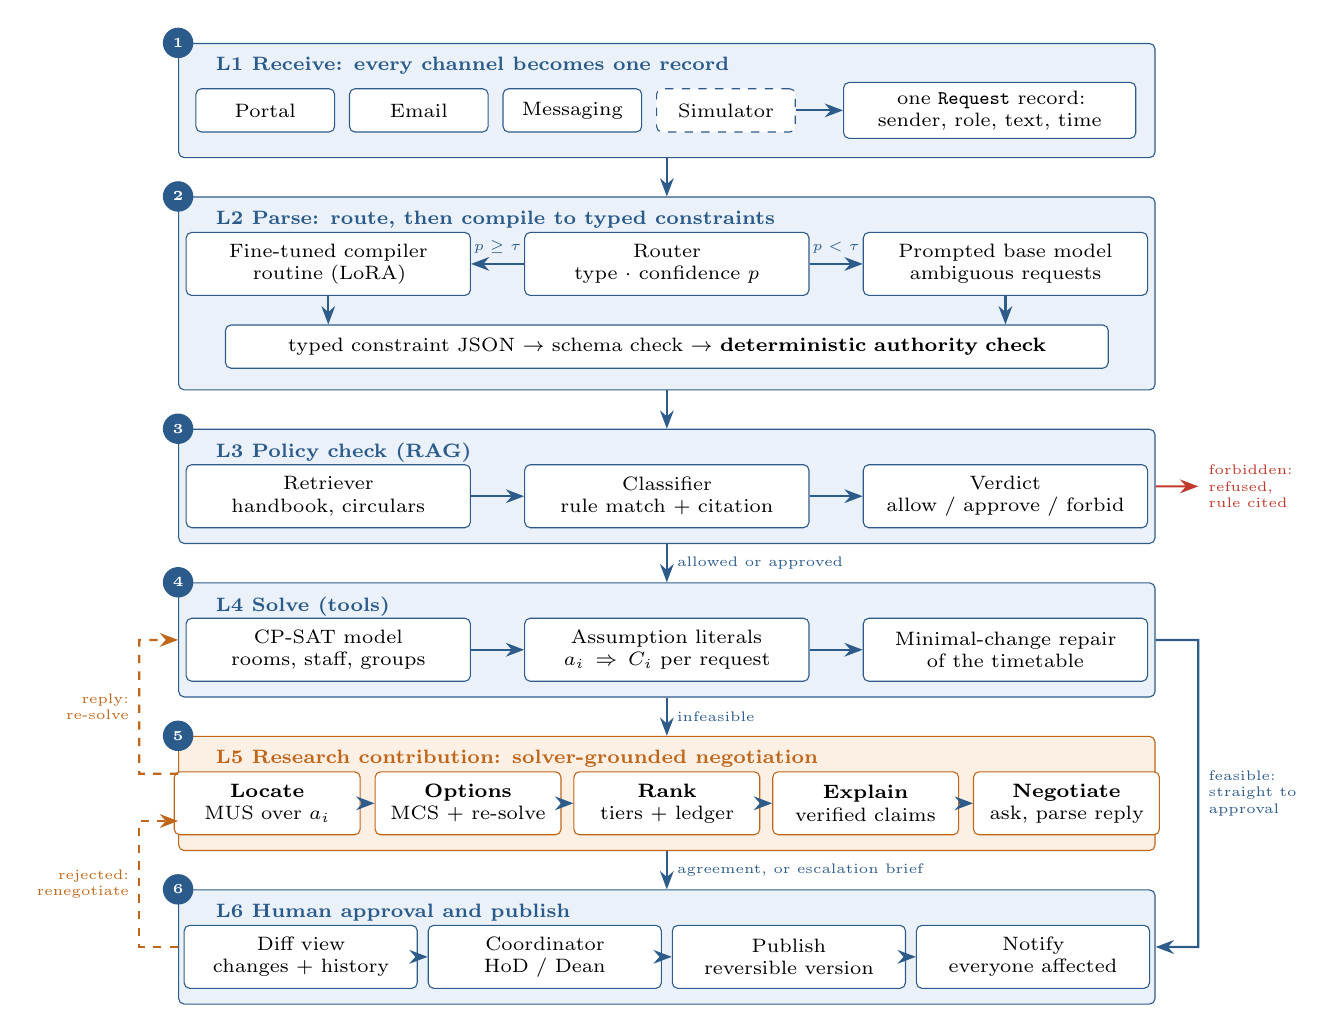
\begin{tikzpicture}[
  band/.style={draw=boxblue,fill=lightblue,rounded corners=2pt,align=center,
    text width=12.1cm,inner sep=4pt,font=\scriptsize},
  box/.style={draw=boxblue,fill=white,rounded corners=2pt,align=center,
    font=\scriptsize,inner sep=3pt,minimum height=0.8cm},
  cbox/.style={box,draw=gaporange,text width=2.15cm},
  badge/.style={circle,fill=secblue,text=white,font=\tiny\bfseries,
    inner sep=0pt,minimum size=11pt},
  ttl/.style={font=\scriptsize\bfseries,anchor=north west},
  note/.style={font=\tiny,text=boxblue,align=center},
  fbnote/.style={font=\tiny,text=gaporange,align=right},
]
  % ---- L1 Receive ----
  \node[box,text width=1.55cm,minimum height=0.55cm] (in1) at (2.9,-2.0) {Portal};
  \node[box,text width=1.55cm,minimum height=0.55cm] (in2) at (4.85,-2.0) {Email};
  \node[box,text width=1.55cm,minimum height=0.55cm] (in3) at (6.8,-2.0) {Messaging};
  \node[box,text width=1.55cm,minimum height=0.55cm,dashed] (in4) at (8.75,-2.0) {Simulator};
  \node[box,text width=3.5cm,minimum height=0.55cm] (rec) at (12.1,-2.0) {one \texttt{Request} record:\\sender, role, text, time};
  \draw[arr] (in4) -- (rec);
  \begin{scope}[on background layer]
    \node[draw=boxblue,fill=lightblue,rounded corners=2pt,inner sep=0pt,
      fit={(1.8,-1.15) (14.2,-2.6)}] (l1) {};
  \end{scope}
  \node[ttl,text=secblue] at (2.15,-1.2) {L1 Receive: every channel becomes one record};

  % ---- L2 Parse ----
  \node[box,text width=3.4cm] (qlora) at (3.7,-3.95) {Fine-tuned compiler\\routine (LoRA)};
  \node[box,text width=3.4cm] (s1)    at (8.0,-3.95) {Router\\type $\cdot$ confidence $p$};
  \node[box,text width=3.4cm] (s2)    at (12.3,-3.95) {Prompted base model\\ambiguous requests};
  \node[box,text width=11.0cm,minimum height=0.55cm] (auth) at (8.0,-5.0)
    {typed constraint JSON $\to$ schema check $\to$ \textbf{deterministic authority check}};
  \begin{scope}[on background layer]
    \node[draw=boxblue,fill=lightblue,rounded corners=2pt,inner sep=0pt,
      fit={(1.8,-3.1) (14.2,-5.55)}] (l2) {};
  \end{scope}
  \node[ttl,text=secblue] at (2.15,-3.15) {L2 Parse: route, then compile to typed constraints};
  \draw[arr] (s1) -- node[above,note] {$p\ge\tau$} (qlora);
  \draw[arr] (s1) -- node[above,note] {$p<\tau$} (s2);
  \draw[arr] (qlora.south) -- (qlora.south |- auth.north);
  \draw[arr] (s2.south) -- (s2.south |- auth.north);
  \draw[arr] (l1.south -| s1) -- (l2.north -| s1);

  % ---- L3 Policy ----
  \node[box,text width=3.4cm] (ret) at (3.7,-6.9) {Retriever\\handbook, circulars};
  \node[box,text width=3.4cm] (cls) at (8.0,-6.9) {Classifier\\rule match + citation};
  \node[box,text width=3.4cm] (out) at (12.3,-6.9) {Verdict\\allow / approve / forbid};
  \draw[arr] (ret) -- (cls);
  \draw[arr] (cls) -- (out);
  \begin{scope}[on background layer]
    \node[draw=boxblue,fill=lightblue,rounded corners=2pt,inner sep=0pt,
      fit={(1.8,-6.05) (14.2,-7.5)}] (l3) {};
  \end{scope}
  \node[ttl,text=secblue] at (2.15,-6.1) {L3 Policy check (RAG)};
  \draw[arr] (l2.south -| s1) -- (l3.north -| s1);

  % ---- L4 Solve ----
  \node[box,text width=3.4cm] (cp)  at (3.7,-8.85) {CP-SAT model\\rooms, staff, groups};
  \node[box,text width=3.4cm] (lit) at (8.0,-8.85) {Assumption literals\\$a_i \Rightarrow C_i$ per request};
  \node[box,text width=3.4cm] (rep) at (12.3,-8.85) {Minimal-change repair\\of the timetable};
  \draw[arr] (cp) -- (lit);
  \draw[arr] (lit) -- (rep);
  \begin{scope}[on background layer]
    \node[draw=boxblue,fill=lightblue,rounded corners=2pt,inner sep=0pt,
      fit={(1.8,-8.0) (14.2,-9.45)}] (l4) {};
  \end{scope}
  \node[ttl,text=secblue] at (2.15,-8.05) {L4 Solve (tools)};
  \draw[arr] (l3.south -| s1) -- node[right,note,align=left] {allowed or approved} (l4.north -| s1);

  % ---- L5 Research contribution ----
  \node[cbox] (a) at (2.925,-10.8) {\textbf{Locate}\\MUS over $a_i$};
  \node[cbox] (b) at (5.475,-10.8) {\textbf{Options}\\MCS + re-solve};
  \node[cbox] (c) at (8.0,-10.8)   {\textbf{Rank}\\tiers + ledger};
  \node[cbox] (d) at (10.525,-10.8){\textbf{Explain}\\verified claims};
  \node[cbox] (e) at (13.075,-10.8){\textbf{Negotiate}\\ask, parse reply};
  \foreach \u/\v in {a/b,b/c,c/d,d/e} \draw[arr] (\u) -- (\v);
  \begin{scope}[on background layer]
    \node[draw=gaporange,fill=gapfill,rounded corners=2pt,inner sep=0pt,
      fit={(1.8,-9.95) (14.2,-11.4)}] (l5) {};
  \end{scope}
  \node[ttl,text=gaporange] at (2.15,-10.0)
    {L5 Research contribution: solver-grounded negotiation};
  \draw[arr] (l4.south -| s1) -- node[right,note,align=left] {infeasible} (l5.north -| s1);

  % ---- L6 Human approval ----
  \node[box,text width=2.75cm] (h1) at (3.35,-12.75) {Diff view\\changes + history};
  \node[box,text width=2.75cm] (h2) at (6.45,-12.75) {Coordinator\\HoD / Dean};
  \node[box,text width=2.75cm] (h3) at (9.55,-12.75) {Publish\\reversible version};
  \node[box,text width=2.75cm] (h4) at (12.65,-12.75) {Notify\\everyone affected};
  \draw[arr] (h1) -- (h2);
  \draw[arr] (h2) -- (h3);
  \draw[arr] (h3) -- (h4);
  \begin{scope}[on background layer]
    \node[draw=boxblue,fill=lightblue,rounded corners=2pt,inner sep=0pt,
      fit={(1.8,-11.9) (14.2,-13.35)}] (l6) {};
  \end{scope}
  \node[ttl,text=secblue] at (2.15,-11.95) {L6 Human approval and publish};
  \draw[arr] (l5.south -| s1) -- node[right,note,align=left] {agreement, or escalation brief} (l6.north -| s1);

  % ---- Paths around the layers ----
  \draw[arr] (l4.east) -- (14.75,-8.725) |- (l6.east)
    node[pos=0.25,right,note,align=left] {feasible:\\straight to\\approval};
  \draw[arr,draw=badred] (l3.east) -- (14.75,-6.775)
    node[right,note,text=badred,align=left] {forbidden:\\refused,\\rule cited};
  \draw[fb] ([yshift=0.25cm]l5.west) -- (1.3,-10.425) |- (l4.west)
    node[pos=0.25,left,fbnote] {reply:\\re-solve};
  \draw[fb] (l6.west) -- (1.3,-12.625) |- ([yshift=-0.35cm]l5.west)
    node[pos=0.25,left,fbnote] {rejected:\\renegotiate};

  \foreach \n/\s in {l1/1,l2/2,l3/3,l4/4,l5/5,l6/6}
    \node[badge] at (\n.north west) {\s};
\end{tikzpicture}}
\caption{Architecture. Solid arrows show the main flow; dashed orange arrows
are feedback loops. The orange layer (L5) is the research contribution.}
\label{fig:arch}
\end{figure}

% ------------------------------------------------------------------
\section{Core Mechanism and Capabilities}
\label{sec:mech}
% ------------------------------------------------------------------
\subsection{Solver-Grounded Negotiation}
\begin{keybox}
\centering
\textbf{Infeasible request} $\;\to\;$ \textbf{MUS} $\;\to\;$ \textbf{MCS}
$\;\to\;$ \textbf{CP-SAT re-solve} $\;\to\;$ \textbf{solver-verified
alternatives} $\;\to\;$ \textbf{negotiation}
\end{keybox}
\noindent Figure~\ref{fig:example} follows one conflict end to end.
\textbf{Constraint model.} Each session is assigned exactly one time slot
and one room, subject to room capacity and type, room occupancy, faculty
availability, student-group clashes and institutional rules. Each
request-derived constraint $C_i$ is guarded by an assumption literal $a_i$,
split into room and slot parts so a repair can relax one without the
other. Protected T0--T2 constraints are guarded too, so they can appear in
explanations, but are never relaxed. Hard constraints are solved first as a
satisfaction problem, where assumption cores apply; preferences are
optimised afterwards.

When the satisfaction stage is infeasible, CP-SAT reports a set of assumption literals
sufficient for infeasibility, which we shrink to a \textbf{minimal
unsatisfiable subset (MUS)}: \emph{where} the conflict is. We then enumerate
a few \textbf{minimal correction sets (MCS)}: minimal sets of constraints
whose removal restores feasibility, i.e.\ \emph{what could give way}.
We enumerate them with our own MARCO-style loop over CP-SAT,
restricted to negotiable literals. An MCS
says which constraints yield, not what the resulting timetable is, so CP-SAT
re-solves each relaxation into a concrete timetable. An option is offered
only if its re-solve succeeds, so \textbf{every compromise a stakeholder
sees is already verified feasible}. Partial concessions (``Thursday afternoon
instead'') weaken a constraint rather than remove it, and trigger another
re-solve. For tractability we cap enumeration at the $K{=}5$ cheapest
candidates per round, fixed before evaluation.

\noindent Four roles are kept separate, which makes this a research question
rather than ``LLM + OR-Tools'':
\begin{table}[H]
\centering\small
\begin{tabularx}{\textwidth}{@{}L{3.6cm} Y@{}}
\toprule
\textbf{Component} & \textbf{Decides}\\
\midrule
Solver (CP-SAT) & \textbf{What is feasible}\\
MCS enumeration & \textbf{What concessions are possible} (the candidate space)\\
Negotiation policy & \textbf{How options rank} (tier, disruption, ledger)\\
LLM & \textbf{Language}: explains, and turns each reply into one typed tool call; never adds a candidate\\
\bottomrule
\end{tabularx}
\end{table}

\subsection{Priority Tiers and Negotiation Policy}
Constraints fall into six published
tiers. \textbf{T0--T2 are protected}: T0 is never relaxed, and any option
touching T1--T2 is escalated to the named authority. \textbf{T3--T5 are
negotiable} under the published priority policy, with priority scores
ordering constraints within a tier.
\begin{table}[H]
\centering\small
\begin{tabularx}{\textwidth}{@{}l L{4.6cm} L{3.4cm} Y@{}}
\toprule
\textbf{Tier} & \textbf{Constraint class} & \textbf{Who may relax it} & \textbf{Example}\\
\midrule
T0 & Physical impossibility & Nobody & Room double-booking; capacity\\
T1 & Institute policy & Dean / council & Max.\ consecutive hours\\
T2 & Institutional commitment & Academic office & Exam blocks; guest windows\\
\midrule
T3 & Verified unavailability & Owner + alternative & Faculty leave\\
T4 & Operational requirement & Owner or HoD & Lab equipment; room type\\
T5 & Preference & Owner, freely & Preferred time; fewer gaps\\
\bottomrule
\end{tabularx}
\end{table}
\textbf{Resolution ladder.} (i)~Try a non-disruptive substitution;
(ii)~re-solve the $K{=}5$ cheapest MCS relaxations; (iii)~rank feasible
options by tier, disruption and increase in burden dispersion; (iv)~ask an
owner of a top-ranked concession; (v)~turn replies into constraints and
re-solve; (vi)~escalate deadlock, timeout or any T1--T2 option. A persistent \textbf{concession ledger} credits each stakeholder who
concedes, making them more expensive to ask next time. Weights are a
published policy, not a claim of objective fairness; we test whether it
spreads burden more evenly than flat weights or free negotiation.
\textbf{Grounded explanations} are contrastive, and each claim must map to
a constraint in the MUS, a cited rule or a solver result; a verifier rejects
unsupported claims. Explanations name the \emph{constraint}, never the
private reason (Figure~\ref{fig:example}).

\subsection{Control Loop, Reply Tools and Safety Boundary}
The resolution ladder is the controller: it ranks options, picks whom to ask
(lowest recent burden), forces T1--T2 escalation and enforces the round
limit. The LLM decides only where free text must be interpreted: each
stakeholder reply (``Thursday, but only after 2'', ``use Lab~3 instead'',
``depends on my TA'') becomes exactly one typed tool call.
\begin{table}[H]
\centering\small
\begin{tabularx}{\textwidth}{@{}l Y@{}}
\toprule
\textbf{Tool (LLM-selected)} & \textbf{Effect and guard}\\
\midrule
\texttt{accept(option\_id)} & Accept an offered option; \texttt{option\_id} is an enum of verified options\\
\texttt{apply\_reply(constraint)} & Weakened or partial constraint; schema/authority-checked, then re-solved\\
\texttt{counter\_propose(option)} & Stakeholder's own alternative; offered onward only if CP-SAT verifies it\\
\texttt{ask\_clarification(question)} & Reply too vague to compile; one follow-up per round\\
\texttt{decline(reason)} & Refusal; the ladder moves to the next-ranked option or owner\\
\texttt{escalate(reason)} & Out of scope, a policy exception or an injected instruction\\
\bottomrule
\end{tabularx}
\end{table}
\noindent A bad call returns a typed error; after two retries the reply
goes to the coordinator. The LLM cannot create candidates, relax T0--T2 or
change state.

\subsection{Five Capabilities: Why Each Is Needed}
\begin{table}[H]
\centering\small
\begin{tabularx}{\textwidth}{@{}L{1.75cm} Y L{5.1cm}@{}}
\toprule
\textbf{Capability} & \textbf{Why the problem needs it} & \textbf{Measured by (vs.\ what)}\\
\midrule
Fine-tuning & Requests arrive continuously and include private staff details, so they must be compiled locally and cheaply; a prompted 2B model misreads local conventions (slot names, lab blocks) & Compilation F1: LoRA Qwen3.5-2B vs prompted 2B vs prompted Gemini Flash\\
RAG & Whether a request is allowed depends on this institute's handbook and circulars, which change each semester and no model knows & Recall@k, citation precision, verdict accuracy, abstention; vs no retrieval\\
Reasoning & Turning a partial reply into a weakened constraint and writing a contrastive explanation are multi-step inferences over the conflict; each step is checked & Claim-level faithfulness, reply-to-constraint accuracy; A2\\
Agentic & Negotiation spans many rounds and people; the ledger is memory across requests; escalation is a hand-off to a human & Resolution rate, rounds, escalation precision; vs B2 (no negotiation)\\
Tool calling & Free-text replies must become the right typed action with valid arguments, and injected text must never trigger an action & Tool-call accuracy, argument validity, recovery, unsafe-action rate; vs A3\\
\bottomrule
\end{tabularx}
\end{table}

\begin{figure}[p]
\centering
\resizebox{\textwidth}{!}{%
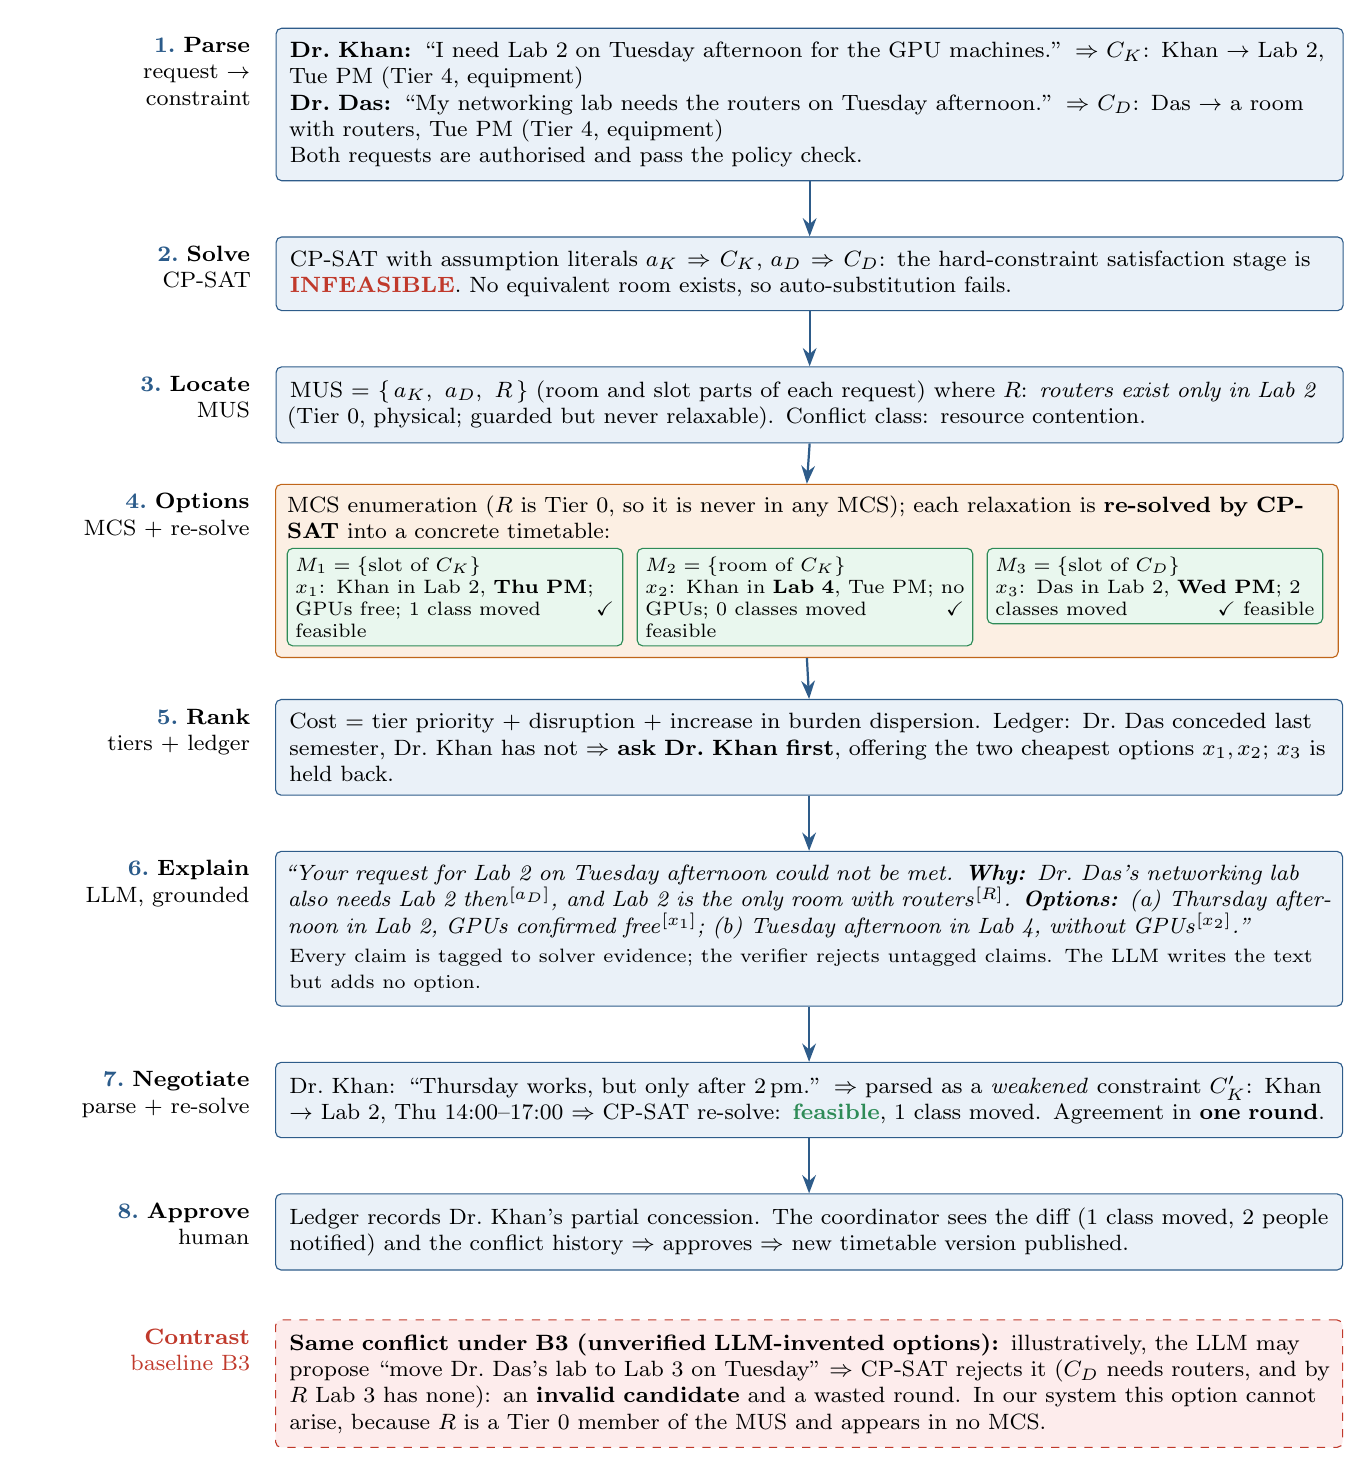
\begin{tikzpicture}[
  cbox/.style={draw=boxblue,fill=lightblue,rounded corners=2pt,align=left,
    text width=13.2cm,inner sep=5pt,font=\footnotesize},
  obox/.style={draw=goodgreen,fill=goodfill,rounded corners=2pt,align=left,
    text width=4.05cm,inner sep=3pt,font=\scriptsize},
  lab/.style={align=right,text width=2.7cm,font=\footnotesize,anchor=north east},
  gap/.style={below=0.7cm of #1.south west,anchor=north west},
]
  % 1 Requests
  \node[cbox,anchor=north west] (C1) at (3.2,0) {%
    \textbf{Dr.\ Khan:} ``I need Lab~2 on Tuesday afternoon for the GPU machines.''
    $\Rightarrow$ $C_K$: Khan $\to$ Lab~2, Tue PM (Tier~4, equipment)\\
    \textbf{Dr.\ Das:} ``My networking lab needs the routers on Tuesday afternoon.''
    $\Rightarrow$ $C_D$: Das $\to$ a room with routers, Tue PM (Tier~4, equipment)\\
    Both requests are authorised and pass the policy check.};
  \node[lab] at ($(C1.north west)+(-0.2,0)$) {\stepno{1}~\textbf{Parse}\\request $\to$ constraint};

  % 2 Solve
  \node[cbox,gap=C1] (C2) {%
    CP-SAT with assumption literals $a_K \Rightarrow C_K$, $a_D \Rightarrow C_D$:
    the hard-constraint satisfaction stage is \textbf{\color{badred}INFEASIBLE}. No equivalent room
    exists, so auto-substitution fails.};
  \node[lab] at ($(C2.north west)+(-0.2,0)$) {\stepno{2}~\textbf{Solve}\\CP-SAT};

  % 3 MUS
  \node[cbox,gap=C2] (C3) {%
    MUS $=\{\,a_K,\; a_D,\; R\,\}$ (room and slot parts of each request) where
    $R$: \emph{routers exist only in Lab~2} (Tier~0, physical; guarded but never
    relaxable). Conflict class: resource contention.};
  \node[lab] at ($(C3.north west)+(-0.2,0)$) {\stepno{3}~\textbf{Locate}\\MUS};

  % 4 MCS + re-solve
  \node[font=\footnotesize,align=left,text width=13.2cm,inner sep=0pt,
    below=0.66cm of C3.south west,anchor=north west,xshift=4pt] (C4t) {%
    MCS enumeration ($R$ is Tier~0, so it is never in any MCS); each
    relaxation is \textbf{re-solved by CP-SAT} into a concrete timetable:};
  \node[obox,below=3pt of C4t.south west,anchor=north west] (o1) {%
    $M_1=\{$slot of $C_K\}$\\ $x_1$: Khan in Lab~2, \textbf{Thu PM};
    GPUs free; 1 class moved \hfill$\checkmark$ feasible};
  \node[obox,right=0.17cm of o1.north east,anchor=north west] (o2) {%
    $M_2=\{$room of $C_K\}$\\ $x_2$: Khan in \textbf{Lab~4}, Tue PM;
    no GPUs; 0 classes moved \hfill$\checkmark$ feasible};
  \node[obox,right=0.17cm of o2.north east,anchor=north west] (o3) {%
    $M_3=\{$slot of $C_D\}$\\ $x_3$: Das in Lab~2, \textbf{Wed PM};
    2 classes moved \hfill$\checkmark$ feasible};
  \begin{scope}[on background layer]
    \node[draw=gaporange,fill=gapfill,rounded corners=2pt,inner sep=4pt,
      fit=(C4t)(o1)(o2)(o3)] (C4) {};
  \end{scope}
  \node[lab] at ($(C4.north west)+(-0.2,0)$) {\stepno{4}~\textbf{Options}\\MCS + re-solve};

  % 5 Rank
  \node[cbox,below=0.52cm of C4.south west,anchor=north west] (C5) {%
    Cost $=$ tier priority $+$ disruption $+$ increase in burden dispersion.
    Ledger: Dr.\ Das conceded last semester, Dr.\ Khan has not
    $\Rightarrow$ \textbf{ask Dr.\ Khan first}, offering the two cheapest
    options $x_1, x_2$; $x_3$ is held back.};
  \node[lab] at ($(C5.north west)+(-0.2,0)$) {\stepno{5}~\textbf{Rank}\\tiers + ledger};

  % 6 Explain
  \node[cbox,gap=C5] (C6) {%
    \emph{``Your request for Lab~2 on Tuesday afternoon could not be met.
    \textbf{Why:} Dr.\ Das's networking lab also needs Lab~2 then}$^{[a_D]}$\emph{,
    and Lab~2 is the only room with routers}$^{[R]}$\emph{. \textbf{Options:}
    (a) Thursday afternoon in Lab~2, GPUs confirmed free}$^{[x_1]}$\emph{;
    (b) Tuesday afternoon in Lab~4, without GPUs}$^{[x_2]}$\emph{.''}\\[1pt]
    {\scriptsize Every claim is tagged to solver evidence; the verifier rejects
    untagged claims. The LLM writes the text but adds no option.}};
  \node[lab] at ($(C6.north west)+(-0.2,0)$) {\stepno{6}~\textbf{Explain}\\LLM, grounded};

  % 7 Reply
  \node[cbox,gap=C6] (C7) {%
    Dr.\ Khan: ``Thursday works, but only after 2\,pm.'' $\Rightarrow$ parsed as a
    \emph{weakened} constraint $C_K'$: Khan $\to$ Lab~2, Thu 14:00--17:00
    $\Rightarrow$ CP-SAT re-solve: \textbf{\color{goodgreen}feasible},
    1 class moved. Agreement in \textbf{one round}.};
  \node[lab] at ($(C7.north west)+(-0.2,0)$) {\stepno{7}~\textbf{Negotiate}\\parse + re-solve};

  % 8 Approve
  \node[cbox,gap=C7] (C8) {%
    Ledger records Dr.\ Khan's partial concession. The coordinator sees the
    diff (1 class moved, 2 people notified) and the conflict history
    $\Rightarrow$ approves $\Rightarrow$ new timetable version published.};
  \node[lab] at ($(C8.north west)+(-0.2,0)$) {\stepno{8}~\textbf{Approve}\\human};

  % B3 contrast
  \node[cbox,draw=badred,fill=badfill,dashed,below=0.62cm of C8.south west,
    anchor=north west] (C9) {%
    \textbf{Same conflict under B3 (unverified LLM-invented options):}
    illustratively, the LLM may propose ``move Dr.\ Das's lab to Lab~3 on Tuesday'' $\Rightarrow$ CP-SAT
    rejects it ($C_D$ needs routers, and by $R$ Lab~3 has none): an \textbf{invalid candidate} and a wasted
    round. In our system this option cannot arise, because $R$ is a Tier~0
    member of the MUS and appears in no MCS.};
  \node[lab,text=badred] at ($(C9.north west)+(-0.2,0)$) {\textbf{Contrast}\\baseline B3};

  \foreach \u/\v in {C1/C2,C2/C3,C3/C4,C4/C5,C5/C6,C6/C7,C7/C8}
    \draw[arr] (\u.south) -- (\v.north);
\end{tikzpicture}}
\vspace{6pt}
\caption{Worked example: one resource-contention conflict, end to end. The
last row shows it under B3; B4 would discard that option and regenerate.
Blue rows are deterministic or solver steps, the
orange row is the MCS candidate space, and only step 6 and the
parsing in steps 1 and 7 use the LLM. Superscripts mark the
solver evidence behind each claim.}
\label{fig:example}
\end{figure}

% ------------------------------------------------------------------
\section{Evaluation}
\label{sec:eval}
% ------------------------------------------------------------------
\small
The primary comparison is ours against B4, which differs \emph{only} in
whether options come from re-solved MCS relaxations or from the LLM plus the
same CP-SAT filter; other systems locate where any gain comes from.

\subsection{Evaluation Environment}
\begin{table}[!htb]
\centering\small
\begin{tabularx}{\textwidth}{@{}L{2.6cm} Y L{2.4cm}@{}}
\toprule
\textbf{Benchmark} & \textbf{Construction} & \textbf{Size}\\
\midrule
\textbf{A. Negotiation} & Synthetic department instances with planted conflicts (resource contention, request vs.\ policy, capacity shortfall); stakeholder simulators with hidden true flexibility; solver-computed oracle outcome & 60 scenarios\\
\textbf{B. Parsing} & Requests generated from known target constraints, then paraphrased, made ambiguous, unauthorised, out-of-scope or adversarial; split by template & 600 (400/49/151)\\
\textbf{C. Policy (RAG)} & Questions over the handbook and circulars labelled with gold rule IDs, plus questions no rule covers (abstention) & 40 + 20 queries\\
\textbf{D. Reply actions} & Stakeholder replies (accept, partial, counter-proposal, vague, refusal, injected instruction) with a known correct call and arguments & 100 replies\\
\bottomrule
\end{tabularx}
\end{table}
Ground truth is known by construction. A 50-case safety set (authority
violations, injections, private-reason requests) and an anonymised human
pilot (5--10 faculty, informed consent, after institutional ethics
clearance) complement the benchmarks.

\textbf{Stakeholder simulators.} Seeded hidden profiles specify acceptable
options (including options outside any MCS) and whether a stakeholder
volunteers an option or replies. Rules decide acceptance from the options
alone; a separate LLM, blind to the negotiator prompt and solver state,
only words the reply. CP-SAT runs single-threaded with a fixed seed, so
paired configurations offer identical options. Four stochastic families (strict, flexible,
cost-sensitive, history-sensitive) test cross-family robustness.

\textbf{Judge validation.} Two team members hand-label 100 explanations
(claim supported or not) and 100 simulator replies; we report Cohen's
$\kappa$ against the faithfulness verifier and the simulator, and report
LLM-scored metrics only where $\kappa\ge0.6$.

\textbf{Models.} All LLM roles use local Qwen3.5-2B Q5\_K\_M (GGUF) via
llama.cpp: prompted for negotiation, explanation, simulation and fallback
parsing; LoRA-tuned for routine compilation. Gemini Flash is the large
prompted parsing reference and re-runs a subset to check model bias.

\subsection{Baselines and Ablations}
\begin{table}[H]
\centering\small
\begin{tabularx}{\textwidth}{@{}l Y l@{}}
\toprule
\textbf{System} & \textbf{How it works} & \textbf{What it isolates}\\
\midrule
B1 LLM-only & LLM writes the timetable directly; no solver & Feasibility gap\\
B2 Solver only & Same model and tiers; imposes the best repair & Value of negotiation\\
B3 Unverified & As ours, but the LLM \emph{invents} options, offered unchecked & Cost of invalid options\\
\textbf{B4 Filtered} & As B3, but CP-SAT filters them; LLM regenerates (${\le}3$ tries) & \textbf{Grounding (RQ)}\\
\textbf{Ours} & Options only from re-solved MCS relaxations & ---\\
Oracle & CP-SAT with all hidden flexibility; no MCS limit & Upper bound\\
\midrule
\multicolumn{3}{@{}l}{\emph{Ablations: one change each, all else fixed}}\\
A1 Flat & Ours with flat stakeholder weights, no tiers or ledger & Fairness (H4)\\
A2 Free text & Ours with free-form instead of evidence-grounded explanations & Grounding (H3)\\
A3 Rule replies & Ours with a keyword/regex reply handler instead of LLM tool calls & Tool calling\\
\bottomrule
\end{tabularx}
\end{table}

\subsection{Evaluation Metrics}
\begin{table}[H]
\centering\small
\begin{tabularx}{\textwidth}{@{}l l Y Y@{}}
\toprule
\textbf{Hyp.} & \textbf{vs.} & \textbf{Primary metrics} & \textbf{Supported if}\\
\midrule
H1 & B3, B4 & Invalid-candidate rate; regeneration calls; extra rounds/escalations & B3 needs more rounds or escalations; B4 more calls\\
H2 & B4, B2 & Resolution rate; rounds if resolved; classes moved; oracle gap & Resolution not lower; fewer rounds, less disruption, smaller gap\\
H3 & A2 & Faithfulness; leaks; text--option mismatches; acceptance & Better on the first three; acceptance not lower\\
H4 & A1 & Burden Gini; max.\ individual burden & Lower dispersion; resolution not lower\\
\bottomrule
\end{tabularx}
\end{table}
\noindent\textbf{Per capability:} compilation F1 (fine-tuning);
recall@k, citation precision, verdict accuracy and abstention (RAG);
claim-level faithfulness and reply-to-constraint accuracy (reasoning);
resolution and escalation precision vs B2 (agentic); tool-call accuracy,
argument validity, error-recovery rate vs A3 (tool calling). \textbf{Safety:}
unsafe or unapproved actions, authority/tier violations, privacy leakage,
injection success.

\smallskip\textbf{Scoring.} Each scenario has one simulator family (balanced
per kind). Ours, B3 and B4 run 60 scenarios $\times$ 3 seeds; A1--A3 run once on
a stratified 30, B1 on 20 (650 LLM runs). A final status that differs from the
oracle's is a \emph{status error} with no oracle gap. Conclusions must hold
across families; each failing run is tagged with its first failing stage.

% ------------------------------------------------------------------
\section{Safety, Compute, Novelty and Risks}
\small
\begin{tcolorbox}[enhanced,colback=lightblue,colframe=boxblue,boxrule=0.8pt,
  arc=3pt,left=6pt,right=6pt,top=2pt,bottom=2pt]
\small
\textbf{Safety.} Every LLM tool call is a proposal that passes \emph{schema validator $\to$
policy + authority $\to$ CP-SAT verify $\to$ human approval} before any
state changes: an architectural invariant, not a prompt
instruction. Messages are untrusted data, so an injection can at worst
produce a proposal the checks or coordinator reject. Private reasons are
never exposed; experiments use synthetic data in a sandboxed database.
\end{tcolorbox}
% ------------------------------------------------------------------
\medskip\noindent\textbf{Compute.} LoRA training of the 2B compiler on $\approx$850 examples takes
$\approx$1--2 GPU-hours per run on a free Kaggle T4 (16\,GB); we budget 3
runs, $\approx$6 GPU-hours. The 650 runs and 100 reply cases need
$\approx$6{,}000 short calls ($\approx$2.5 GPU-hours at $\approx$1.5\,s on a
T4): $\approx$9 GPU-hours in total; the solver runs on a CPU.
Gemini Flash (parsing reference on 151 requests; ours vs B4
on 20 scenarios to check model bias) needs $\approx$600 free-tier calls (\$0).

\medskip\noindent\textbf{Expected novelty.} (1)~\emph{Solver-grounded negotiation:}
LLM + solver systems verify what the LLM proposes; we let MCS enumeration
define the candidate space and measure the difference against
generate-and-filter (H1--H2). (2)~\emph{Concession-aware policy:} published
tiers set who may relax what, and a ledger carries concessions across
requests and semesters, judged by burden spread (H4). (3)~\emph{Grounded,
private explanations:} every claim traces to the conflict set, a rule or a
solver result, checked claim by claim, with private reasons withheld (H3).

\medskip\noindent\textbf{Risks $\to$ fallbacks.} MCS enumeration expensive $\to$
restrict to the affected sub-problem, cap $K$. MCS misses acceptable options
$\to$ admit verified stakeholder proposals; report the loss via oracle gap.
Simulators biased or sharing a model $\to$ four families, rule-decided
acceptance, Gemini Flash cross-check. Fine-tuned parser underperforms $\to$
prompted model; report the negative result. 2B model misreads replies
$\to$ grammar-constrained calls, coordinator fallback. Schedule slips $\to$ cut the
router, then A3, then the pilot; never Ours vs B4.
\end{document}
